\pdfoutput=1
% Options for packages loaded elsewhere
\PassOptionsToPackage{unicode}{hyperref}
\PassOptionsToPackage{hyphens}{url}
\PassOptionsToPackage{dvipsnames,svgnames,x11names}{xcolor}
%
\documentclass[
  11pt]{article}
\usepackage{amsmath,amssymb}
\usepackage{iftex}
\ifPDFTeX
  \usepackage[T1]{fontenc}
  \usepackage[utf8]{inputenc}
  \usepackage{textcomp} % provide euro and other symbols
\else % if luatex or xetex
  \usepackage{unicode-math} % this also loads fontspec
  \defaultfontfeatures{Scale=MatchLowercase}
  \defaultfontfeatures[\rmfamily]{Ligatures=TeX,Scale=1}
\fi
\usepackage{lmodern}
\ifPDFTeX\else
  % xetex/luatex font selection
\fi
% Use upquote if available, for straight quotes in verbatim environments
\IfFileExists{upquote.sty}{\usepackage{upquote}}{}
\IfFileExists{microtype.sty}{% use microtype if available
  \usepackage[]{microtype}
  \UseMicrotypeSet[protrusion]{basicmath} % disable protrusion for tt fonts
}{}
\makeatletter
\@ifundefined{KOMAClassName}{% if non-KOMA class
  \IfFileExists{parskip.sty}{%
    \usepackage{parskip}
  }{% else
    \setlength{\parindent}{0pt}
    \setlength{\parskip}{6pt plus 2pt minus 1pt}}
}{% if KOMA class
  \KOMAoptions{parskip=half}}
\makeatother
\usepackage{xcolor}
\usepackage{color}
\usepackage{fancyvrb}
\newcommand{\VerbBar}{|}
\newcommand{\VERB}{\Verb[commandchars=\\\{\}]}
\DefineVerbatimEnvironment{Highlighting}{Verbatim}{commandchars=\\\{\}}
% Add ',fontsize=\small' for more characters per line
\newenvironment{Shaded}{}{}
\newcommand{\AlertTok}[1]{\textcolor[rgb]{1.00,0.00,0.00}{\textbf{#1}}}
\newcommand{\AnnotationTok}[1]{\textcolor[rgb]{0.38,0.63,0.69}{\textbf{\textit{#1}}}}
\newcommand{\AttributeTok}[1]{\textcolor[rgb]{0.49,0.56,0.16}{#1}}
\newcommand{\BaseNTok}[1]{\textcolor[rgb]{0.25,0.63,0.44}{#1}}
\newcommand{\BuiltInTok}[1]{\textcolor[rgb]{0.00,0.50,0.00}{#1}}
\newcommand{\CharTok}[1]{\textcolor[rgb]{0.25,0.44,0.63}{#1}}
\newcommand{\CommentTok}[1]{\textcolor[rgb]{0.38,0.63,0.69}{\textit{#1}}}
\newcommand{\CommentVarTok}[1]{\textcolor[rgb]{0.38,0.63,0.69}{\textbf{\textit{#1}}}}
\newcommand{\ConstantTok}[1]{\textcolor[rgb]{0.53,0.00,0.00}{#1}}
\newcommand{\ControlFlowTok}[1]{\textcolor[rgb]{0.00,0.44,0.13}{\textbf{#1}}}
\newcommand{\DataTypeTok}[1]{\textcolor[rgb]{0.56,0.13,0.00}{#1}}
\newcommand{\DecValTok}[1]{\textcolor[rgb]{0.25,0.63,0.44}{#1}}
\newcommand{\DocumentationTok}[1]{\textcolor[rgb]{0.73,0.13,0.13}{\textit{#1}}}
\newcommand{\ErrorTok}[1]{\textcolor[rgb]{1.00,0.00,0.00}{\textbf{#1}}}
\newcommand{\ExtensionTok}[1]{#1}
\newcommand{\FloatTok}[1]{\textcolor[rgb]{0.25,0.63,0.44}{#1}}
\newcommand{\FunctionTok}[1]{\textcolor[rgb]{0.02,0.16,0.49}{#1}}
\newcommand{\ImportTok}[1]{\textcolor[rgb]{0.00,0.50,0.00}{\textbf{#1}}}
\newcommand{\InformationTok}[1]{\textcolor[rgb]{0.38,0.63,0.69}{\textbf{\textit{#1}}}}
\newcommand{\KeywordTok}[1]{\textcolor[rgb]{0.00,0.44,0.13}{\textbf{#1}}}
\newcommand{\NormalTok}[1]{#1}
\newcommand{\OperatorTok}[1]{\textcolor[rgb]{0.40,0.40,0.40}{#1}}
\newcommand{\OtherTok}[1]{\textcolor[rgb]{0.00,0.44,0.13}{#1}}
\newcommand{\PreprocessorTok}[1]{\textcolor[rgb]{0.74,0.48,0.00}{#1}}
\newcommand{\RegionMarkerTok}[1]{#1}
\newcommand{\SpecialCharTok}[1]{\textcolor[rgb]{0.25,0.44,0.63}{#1}}
\newcommand{\SpecialStringTok}[1]{\textcolor[rgb]{0.73,0.40,0.53}{#1}}
\newcommand{\StringTok}[1]{\textcolor[rgb]{0.25,0.44,0.63}{#1}}
\newcommand{\VariableTok}[1]{\textcolor[rgb]{0.10,0.09,0.49}{#1}}
\newcommand{\VerbatimStringTok}[1]{\textcolor[rgb]{0.25,0.44,0.63}{#1}}
\newcommand{\WarningTok}[1]{\textcolor[rgb]{0.38,0.63,0.69}{\textbf{\textit{#1}}}}
\usepackage{longtable,booktabs,array}
\usepackage{calc} % for calculating minipage widths
% Correct order of tables after \paragraph or \subparagraph
\usepackage{etoolbox}
\makeatletter
\patchcmd\longtable{\par}{\if@noskipsec\mbox{}\fi\par}{}{}
\makeatother
% Allow footnotes in longtable head/foot
\IfFileExists{footnotehyper.sty}{\usepackage{footnotehyper}}{\usepackage{footnote}}
\makesavenoteenv{longtable}
\usepackage{graphicx}
\makeatletter
\def\maxwidth{\ifdim\Gin@nat@width>\linewidth\linewidth\else\Gin@nat@width\fi}
\def\maxheight{\ifdim\Gin@nat@height>\textheight\textheight\else\Gin@nat@height\fi}
\makeatother
% Scale images if necessary, so that they will not overflow the page
% margins by default, and it is still possible to overwrite the defaults
% using explicit options in \includegraphics[width, height, ...]{}
\setkeys{Gin}{width=\maxwidth,height=\maxheight,keepaspectratio}
% Set default figure placement to htbp
\makeatletter
\def\fps@figure{htbp}
\makeatother
\setlength{\emergencystretch}{3em} % prevent overfull lines
\providecommand{\tightlist}{%
  \setlength{\itemsep}{0pt}\setlength{\parskip}{0pt}}
\setcounter{secnumdepth}{-\maxdimen} % remove section numbering
\ifLuaTeX
\usepackage[bidi=basic]{babel}
\else
\usepackage[bidi=default]{babel}
\fi
\babelprovide[main,import]{american}
% get rid of language-specific shorthands (see #6817):
\let\LanguageShortHands\languageshorthands
\def\languageshorthands#1{}
\usepackage[T1]{fontenc}
\usepackage[utf8]{inputenc}
\usepackage{lmodern}
\usepackage{microtype}
\usepackage{booktabs,longtable,array,ragged2e,graphicx,float,caption,xcolor,enumitem}
\usepackage{geometry}
\geometry{letterpaper,top=0.82in,bottom=0.86in,left=0.92in,right=0.92in}
\captionsetup{font=small,labelfont=bf}
\setlength{\parindent}{0pt}
\setlength{\parskip}{0.52em}
\setlength{\emergencystretch}{3em}
\setlist{nosep,leftmargin=*}
\AtBeginEnvironment{longtable}{\small}
\usepackage{newunicodechar}
\newunicodechar{δ}{\ensuremath{\delta}}
\newunicodechar{ρ}{\ensuremath{\rho}}
\newunicodechar{×}{\ensuremath{\times}}
\newunicodechar{→}{\ensuremath{\rightarrow}}
\newunicodechar{−}{\ensuremath{-}}
\ifLuaTeX
  \usepackage{selnolig}  % disable illegal ligatures
\fi
\IfFileExists{bookmark.sty}{\usepackage{bookmark}}{\usepackage{hyperref}}
\IfFileExists{xurl.sty}{\usepackage{xurl}}{} % add URL line breaks if available
\urlstyle{same}
\hypersetup{
  pdftitle={Passing Coarse Marginal Checks Can Be Cheap: Persona Mixtures and Imprecise Treatment-Response Estimates in an LLM Persona Panel},
  pdfauthor={Yohei Nakajima},
  pdflang={en-US},
  colorlinks=true,
  linkcolor={blue},
  filecolor={Maroon},
  citecolor={Blue},
  urlcolor={blue},
  pdfcreator={LaTeX via pandoc}}

\title{Passing Coarse Marginal Checks Can Be Cheap: Persona Mixtures and
Imprecise Treatment-Response Estimates in an LLM Persona Panel}
\author{Yohei Nakajima}
\date{Untapped Capital - July 2026}

\begin{document}
\maketitle

\begin{abstract}
Large language models are increasingly used as synthetic research participants and are often validated by whether their marginal responses resemble human data. We study a fixed panel of sixteen lightweight persona-conditioned GPT-4.1 configurations in repeated strategic games. The panel passed preregistered broad-reference checks in three of four repeated-game cells. A fixed-panel Dirichlet-Jeffreys sensitivity places median between-prompt shares of episode-level variation at 63%-71% (95% intervals 49%-81%); finite-opportunity plug-in estimates are 85%-96%. Aggregate continuation-probability contrasts are +0.083 and +0.078, with conservative simultaneous 95% intervals [-0.171, +0.330] and [-0.181, +0.330]. The treatment changed both continuation probability and its textual representation, so incentive and framing channels remain undecomposed. Separate representation experiments found that replacing and repositioning one sentence shifted cooperation from 0/40 to 37/40 in a bare configuration, and that a displayed label or learned label-linked prior could override payoff dominance in one conflict cell. External review exposed family-error, dependence, and boundary-uncertainty defects; zero-call reanalysis changed the interpretation while preserving the historical record. A public capsule verifies 4,916 confirmatory Phase 3-5 runs with no live model calls. The results concern one model-prompt panel, use protocol-nonmatched human references, and do not establish human substitutability.
\end{abstract}

\hypertarget{introduction}{%
\subsection{1. Introduction}\label{introduction}}

Human behavioral experiments are slow and expensive; LLM calls are fast
and nearly free. A growing literature reports that suitably conditioned
LLMs produce data resembling human data---``algorithmic fidelity''
{[}Argyle et al.~2023{]}, ``homo silicus'' {[}Horton 2023{]}, behavior
``statistically indistinguishable from a random human'' {[}Mei et
al.~2024{]}---and a formal framework for evaluating \emph{statistical
realism} now exists {[}Xie et al.~2026{]}. Much of this evidence
validates marginals: means, distributions, and aggregate replication.

Recent work shows that descriptive realism and causal fidelity can
diverge at scale {[}Li \& Ji 2026{]}, that treating LLM outcomes as
surrogates for human outcomes requires assumptions that marginal
equivalence does not supply {[}Persson et al.~2026{]}, and that
intervention prompts can shift a model's implied latent user even when
explicit persona text is fixed {[}Lin et al.~2026{]}. Li and Ji
additionally trace effect errors to intervention logic, outcome
structure, and excessive attitude--behavior coupling, so the present
paper does not claim mechanism-level explanation in general. Its
narrower contribution is a specific fixed-panel composition mechanism in
incentive-bearing strategic interaction, coupled to minimal
representation interventions and an auditable correction record. We
decompose the explicit persona panel into between-prompt dispersion,
within-prompt variation, and prompt-indexed treatment response. The
panel passes coarse marginal checks while producing small but
imprecisely estimated continuation-probability contrasts, and most
recorded variation lies between prompt configurations rather than within
them. Sealed templates and matched procedures control explicit
assignment, environment randomization, and execution. They do not
establish latent-person invariance; Lin-style user drift and the
observed composition pattern can coexist.

Here, ``cheap'' denotes evidentiary economy rather than only low API
cost: the broad-reference marginal checks could be passed without
estimating the treatment-response object they might be taken to
validate.

\textbf{Contributions.} First, we provide a registered
strategic-interaction example in which a fixed persona panel passes
coarse condition-level and dispersion checks while aggregate
continuation-probability point differences remain imprecisely estimated;
the design does not establish equivalence or a narrow response bound
(§4.1). Second, we quantify the associated composition problem with
three explicitly different uncertainty views: a fixed-panel
latent-propensity posterior, finite-opportunity plug-in estimates, and
an exploratory persona-generator bootstrap; the first places median
between-prompt shares at 63\%--71\%, while representation experiments
show how wording and displayed labels or learned game priors govern the
induced policies (§4.1--4.3). Third, we demonstrate an auditable
reliability protocol---and its limits---through prospective
registration, external chronology, mechanical adjudication, complete
zero-call replay of the confirmatory record, and public correction of
family-error and construct-validity defects (§4.4--4.5).

\hypertarget{related-work}{%
\subsection{2. Related work}\label{related-work}}

\textbf{Occupied territory, and where we sit.} Li and Ji {[}2026{]}
establish across three model families, eleven interventions, and 59,508
participants that descriptive fit and intervention-effect accuracy can
diverge, that prompt refinements improving realism do not reliably
improve effect accuracy, and that errors vary with intervention logic,
outcome structure, and attitude--behavior coupling. Persson,
Schultzberg, and Ankargren {[}2026{]} formalize when LLM outcomes can
serve as causal surrogates and why novel interventions still require
human evidence. Lin et al.~{[}2026{]} show that interventions can change
the implicit simulated population even when explicit personas are fixed.
Statistical-realism, persona-collapse, and state-versus-trait work
further show that persona-conditioned populations can compress or
misallocate heterogeneity {[}Xie et al.~2026; Harry et al.~2026; Xiao et
al.~2026{]}. Our differentiation is therefore not the broad divergence
or the existence of mechanisms. It is a registered decomposition of one
common lightweight construction in strategic interaction: the same fixed
explicit prompt panel is evaluated for marginal fit,
finite-opportunity-corrected between/within composition, representation
sensitivity, and response to a represented continuation-probability
treatment, with exact prompt provenance and public inferential
correction. The observed composition pattern is complementary to, not
exclusive of, latent-user drift.

\textbf{LLM strategic behavior.} Akata et al.~{[}2025{]} characterize
repeated-game play modulated by prompts; Pal et al.~{[}2026{]} elicit
strategies from five models while varying continuation probability,
payoffs, horizon knowledge, and framing; counterfactual-reasoning
evaluations alter labels and payoff structures {[}Georgousis et
al.~2026{]}; and ``strategic robustness'' has been defined as
payoff-preserving invariance across narratives {[}Mousavi Davoudi et
al.~2026{]}. These works establish that neither repeated games nor
prompt/payoff perturbations are new. Our distinct combination is the
fixed persona panel, the explicit between/within/response decomposition,
exact prompt provenance, prospective registration of confirmatory
claims, and mechanical adjudication followed by public inferential
correction.

\textbf{Strong positive evidence, and a different estimand.} Ashokkumar,
Hewitt, Ghezae, and Willer {[}2026{]} use study descriptions to forecast
469 effects from 70 preregistered, nationally representative survey
experiments and find strong correlations with realized effects,
alongside systematic effect-size overestimation and weaker performance
in a megastudy archive. That is important contrary evidence against any
blanket pessimism about LLMs in experimental science. It is also a
forecasting task over studies rather than subject-level simulation of a
response surface. Strong effect forecasting is compatible with the
fixed-panel composition failure studied here and reinforces the
prescription to validate a simulator on the exact response object for
which it will be used.

\textbf{Synthetic participants and personas.} Bisbee et al.~{[}2024{]}
find plausible survey averages alongside compressed variance, distorted
coefficients, and temporal drift; Boelaert et al.~{[}2025{]} report
excess homogeneity; Anthis et al.~{[}2025{]} catalog diversity and
generalization challenges; Hullman et al.~{[}2026{]} propose statistical
calibration for confirmatory use; and Park et al.~{[}2024{]} show that
rich interview conditioning can substantially outperform lightweight
demographic/persona descriptions. Format sensitivity {[}Sclar et
al.~2024{]}, role-play framing {[}Shanahan et al.~2023{]}, persona
collapse {[}Xiao et al.~2026{]}, state blindness {[}Harry et
al.~2026{]}, and reviews of persona-experiment transparency {[}Batzner
et al.~2025{]} all caution against treating a persona string as a stable
human analogue. RLHF-related diversity reduction is a possible mechanism
for concentrated policies, not a mechanism identified by this design.
Full map: \texttt{docs/analysis/literature-map.md}; differentiation
table: \texttt{docs/analysis/novelty-relationships.md}.

\hypertarget{instrument-and-inferential-units}{%
\subsection{3. Instrument and inferential
units}\label{instrument-and-inferential-units}}

The primary deployment is gpt-4.1 with 16-token outputs and a fixed
minimal behavioral-subject prompt containing no game-theory vocabulary
or reasoning scaffold. Temperature was 0.7 except in the registered
Phase 5 sweep at 1.0 and 1.3. On the primary OpenAI-compatible path,
\texttt{temperature} and \texttt{max\_tokens=16} were explicitly
supplied; the assembled prompt set \texttt{top\_p=1.0}, which the
adapter intentionally omitted from the wire at 1.0, while
\texttt{presence\_penalty}, \texttt{frequency\_penalty}, and
\texttt{logit\_bias} were not supplied and therefore inherited provider
defaults. No tools or native structured output were used. Phase 5
prepends one sealed persona sentence to byte-identical task text. The
cross-vendor Gemini tier is descriptive; the original Claude Haiku
candidate failed a registered entry gate and was replaced under an
archived amendment. Environment randomness is seeded; provider-side
generation is not claimed to be seeded. Every request, rendered prompt,
completion, decoding configuration, round, and provenance record is
archived.

\hypertarget{sequential-architecture-and-registration-status}{%
\subsubsection{3.1 Sequential architecture and registration
status}\label{sequential-architecture-and-registration-status}}

\begin{longtable}[]{@{}
  >{\raggedright\arraybackslash}p{(\columnwidth - 6\tabcolsep) * \real{0.2500}}
  >{\raggedright\arraybackslash}p{(\columnwidth - 6\tabcolsep) * \real{0.2500}}
  >{\raggedright\arraybackslash}p{(\columnwidth - 6\tabcolsep) * \real{0.2500}}
  >{\raggedright\arraybackslash}p{(\columnwidth - 6\tabcolsep) * \real{0.2500}}@{}}
\toprule\noalign{}
\begin{minipage}[b]{\linewidth}\raggedright
Stage
\end{minipage} & \begin{minipage}[b]{\linewidth}\raggedright
Primary question and role
\end{minipage} & \begin{minipage}[b]{\linewidth}\raggedright
Unit used in the paper
\end{minipage} & \begin{minipage}[b]{\linewidth}\raggedright
Registration status
\end{minipage} \\
\midrule\noalign{}
\endhead
\bottomrule\noalign{}
\endlastfoot
Phase 1 & Initial prototype and naive behavioral claims; establishes the
historical baseline, not current confirmatory evidence & provider calls
/ recorded decisions & post hoc instrument development \\
Phase 2 & Mechanical re-adjudication and enforcement repair after the
initial harness exposed analyst discretion & archived runs and claim
predicates & corrective, not prospective confirmation \\
Phase 3 & Bare GPT-4.1 configuration in repeated PD, framing, and RPS &
episode, with historical seat-level summaries disclosed & claims
registered before Phase 3 data \\
Phase 4 & Representation robustness, X1/X2 wording extensions,
counterfactual payoffs/labels, continuation-probability assays,
adversaries, and sentinels & complete episode for current sensitivities
& X1 was a sequentially registered, result-informed extension: Phase 3
motivated the test, while its prompts, sample size, and predicate were
sealed before any X1 data; the remaining blocks were registered before
their own data \\
Phase 5 & Sixteen sealed persona-prefix configurations crossed with the
Phase 4 instruments; descriptive Gemini tier & complete persona prompt
for the fixed panel; episode beneath it & confirmatory predicates
registered before Phase 5 data; post-adjudication sensitivities are
explicitly unregistered \\
\end{longtable}

The present paper's main empirical decomposition is Phase 5, interpreted
using representation results from Phases 3--4. Phases 1--2 document
instrument evolution and are not counted as prospective confirmation.

The full event store contains 5,505 completed runs, 54,276 round events,
108,552 seat-round decisions, and 36,251 archived provider-request
events. The public confirmatory replay contract now verifies 4,916 Phase
3--5 runs: 320 registered Phase 3/X1 LLM runs, 20 deterministic Phase 3
baselines, 2,864 Phase 4 runs, and 1,712 Phase 5 runs; three additional
completed legacy entry/diagnostic runs are also replayed but are not
counted as confirmatory. A separate transactional ledger records 30,530
Phase 4--5 calls, 13,141,675 input tokens, and 45,247 output tokens; it
excludes earlier phases and therefore must not be conflated with the
full event-store request count. Counts and definitions are reconciled in
\texttt{docs/analysis/submission/count-reconciliation.md}.

Confirmatory claims were registered before the data that adjudicated
them and were mechanically evaluated in a fixed vocabulary. The
historical two-sided interiority rule used Clopper--Pearson bounds on
seat-level round-one trials. Because two seats share an episode, the
submission analysis additionally treats the complete episode as the
independence unit. For an episode outcome \(Y\in\{0,0.5,1\}\), the
conservative exact sensitivity writes

\[
Y=\tfrac12\{\mathbf 1(Y\ge0.5)+\mathbf 1(Y=1)\},
\]

constructs simultaneous Clopper--Pearson intervals for the two
episode-level binary components, and projects them onto \(E[Y]\). For
wording family \(w\), prompt \(i\), continuation condition \(d\), and
six complete episodes \(e\), define \(A_{ide}=\mathbf 1(Y_{ide}\ge .5)\)
and \(B_{ide}=\mathbf 1(Y_{ide}=1)\), so
\(\hat p_i(d)=\{\bar A_i(d)+\bar B_i(d)\}/2\). For each aggregate
contrast, the sixteen equally weighted prompt cells contribute 96
episodes per condition; pooled component counts therefore estimate
\(\bar p(d)=16^{-1}\sum_i p_i(d)\). The four component-condition
intervals split the total error rate by Bonferroni. If \([L_d,U_d]\) is
the projected condition-mean interval, the contrast interval is

\[
[L_{.90}-U_{.10},\;U_{.90}-L_{.10}].
\]

Under the pooled independent-binomial component model this union-bound
construction has at least 95\% simultaneous coverage; with independent
heterogeneous prompt probabilities the component totals are
Poisson-binomial and no more dispersed than the equal-probability
binomial at the same mean, making the binomial projection conservative
for that working model; its role is a conservative small-sample
projection rather than a claim that the sixteen prompt propensities are
homogeneous. It does not assume seat independence and does not collapse
to zero uncertainty when all observed episodes agree. A
Dirichlet--Jeffreys sensitivity uses the symmetric Dirichlet(0.5, 0.5,
0.5) prior on the probabilities of episode outcomes \{0, 0.5, 1\};
posterior draws project \(E[Y]=0.5q_{0.5}+q_1\). The percentile cluster
bootstrap is also retained as a post-adjudication sensitivity. The exact
Clopper--Pearson projection is the conservative reference because it
provides finite-sample coverage for the discrete episode mean; at n=6
the percentile bootstrap has no comparable coverage guarantee and can
understate uncertainty. Its degeneracy at exact corners is a symptom of
that limitation, not by itself a false-positive mechanism for this
strict interiority gate.

The hierarchy is deployment → explicit persona prompt → condition →
episode → seat → round → provider request. Phase 5's confirmatory unit
is the complete persona sentence; name, age, occupation, and traits are
bundled semantic treatments. Registered claims attach to the conditional
finite-panel estimand for these sixteen prompts. Claims about a wider
persona generator are exploratory at \(n=16\). Pairing the same explicit
prompt across conditions identifies a prompt-indexed contrast, not
necessarily a stable latent person's treatment effect.

\textbf{Protocol glossary.} \texttt{S2-absent} and \texttt{S2-present}
are the registered repeated-game wording families.
\textbf{switch-bearing} means the span whose adjacent substitution
produced the largest preregistered ladder gap and subsequently passed
held-out confirmation; S2-present contains that
replacement-and-reposition operation, while S2-absent contains the
original sentence. \texttt{P3-A3} is the Phase 3 registered
broad-reference cooperation claim, with band {[}0.36, 0.63{]}.
\texttt{P5-1a}, historically called the \textbf{corner-mixture
predicate}, is the registered support condition that fires when the
interior fraction in the exact-bare-twin restricted set is below 0.10
under the frozen seat-level rule; it is not a general theorem about
mixture structure. \texttt{P5-1b} is the registered between-persona
dispersion comparison. \texttt{P5-2} pools registered conflict cells and
classifies whether choices follow task text or persona-conditioned
direction. \texttt{P5-3(a)}---clause (a)---asks whether any persona ×
wording pair has both continuation-probability cells interior and a
positive slope lower bound; \texttt{P5-3(b)}---clause (b)---asks whether
each persona lane rejects the bare configuration's dominated swap-cell
option at a registered minimum rate. Historical verdict labels remain
visible even where post-adjudication analyses change their scientific
interpretation.

\textbf{Phase 5 condition matrix.} The 96 Tier-A persona--condition
units are the full cross of sixteen prompts with six conditions:

\begin{longtable}[]{@{}
  >{\raggedright\arraybackslash}p{(\columnwidth - 4\tabcolsep) * \real{0.3333}}
  >{\raggedright\arraybackslash}p{(\columnwidth - 4\tabcolsep) * \real{0.3333}}
  >{\raggedright\arraybackslash}p{(\columnwidth - 4\tabcolsep) * \real{0.3333}}@{}}
\toprule\noalign{}
\begin{minipage}[b]{\linewidth}\raggedright
Code
\end{minipage} & \begin{minipage}[b]{\linewidth}\raggedright
Condition
\end{minipage} & \begin{minipage}[b]{\linewidth}\raggedright
Role in the paper
\end{minipage} \\
\midrule\noalign{}
\endhead
\bottomrule\noalign{}
\endlastfoot
\texttt{rep-d10-s2a} & repeated PD, δ=.10, S2 absent & repeated-game
level, variance, and response \\
\texttt{rep-d10-s2p} & repeated PD, δ=.10, S2 present & repeated-game
level, variance, and response \\
\texttt{rep-d90-s2a} & repeated PD, δ=.90, S2 absent & repeated-game
level, variance, and response \\
\texttt{rep-d90-s2p} & repeated PD, δ=.90, S2 present & repeated-game
level, variance, and response \\
\texttt{os-swap} & one-shot canonical-payoff label swap &
semantic-label/payoff conflict \\
\texttt{os-community} & one-shot Community framing & near-interior
framing anchor \\
\end{longtable}

The registered P5-1a concept restricted its primary denominator to
persona cells whose \textbf{exact recorded bare twin} failed the same
interiority gate. An outcome-blind exact-twin completion fixed that set
as \texttt{rep-d90-s2a} and \texttt{os-swap}: sixteen personas in each
condition, hence 32 units. The exact Community twin passed the bare
gate; the other three repeated-game cells lacked exact bare twins and
entered only the unrestricted 96-cell secondary.

The machinery's boundary is explicit:

\begin{quote}
\textbf{The pipeline can enforce a registered predicate exactly; it
cannot guarantee that the predicate represents a valid estimand, test
family, or construct.}
\end{quote}

\hypertarget{results}{%
\subsection{4. Results}\label{results}}

\hypertarget{coarse-marginal-checks-pass-while-represented-treatment-estimates-remain-imprecise}{%
\subsubsection{4.1 Coarse marginal checks pass while
represented-treatment estimates remain
imprecise}\label{coarse-marginal-checks-pass-while-represented-treatment-estimates-remain-imprecise}}

The preregistered leaning rule---at least two of agreeable, patient, and
risk-averse---divides the fixed panel into eight cooperative-leaning and
eight defect-leaning complete prompts. The descriptive gaps range from
0.510 to 0.719 across every non-swap condition:

\begin{longtable}[]{@{}
  >{\raggedright\arraybackslash}p{(\columnwidth - 8\tabcolsep) * \real{0.1579}}
  >{\raggedleft\arraybackslash}p{(\columnwidth - 8\tabcolsep) * \real{0.2105}}
  >{\raggedleft\arraybackslash}p{(\columnwidth - 8\tabcolsep) * \real{0.2105}}
  >{\raggedleft\arraybackslash}p{(\columnwidth - 8\tabcolsep) * \real{0.2105}}
  >{\raggedleft\arraybackslash}p{(\columnwidth - 8\tabcolsep) * \real{0.2105}}@{}}
\toprule\noalign{}
\begin{minipage}[b]{\linewidth}\raggedright
condition
\end{minipage} & \begin{minipage}[b]{\linewidth}\raggedleft
cooperative-leaning mean
\end{minipage} & \begin{minipage}[b]{\linewidth}\raggedleft
defect-leaning mean
\end{minipage} & \begin{minipage}[b]{\linewidth}\raggedleft
difference
\end{minipage} & \begin{minipage}[b]{\linewidth}\raggedleft
prompts per stratum
\end{minipage} \\
\midrule\noalign{}
\endhead
\bottomrule\noalign{}
\endlastfoot
\texttt{rep-d10-s2a} & 0.615 & 0.083 & +0.531 & 8 \\
\texttt{rep-d10-s2p} & 0.760 & 0.094 & +0.667 & 8 \\
\texttt{rep-d90-s2a} & 0.688 & 0.177 & +0.510 & 8 \\
\texttt{rep-d90-s2p} & 0.865 & 0.146 & +0.719 & 8 \\
\texttt{os-community} & 0.688 & 0.019 & +0.669 & 8 \\
\end{longtable}

These are fixed-panel prompt-bundle contrasts, not causal estimates for
any trait. The P3-A3 broad-reference cooperation band is {[}0.36,
0.63{]}. The four repeated-game pool means are 0.349
(\texttt{rep-d10-s2a}), 0.427 (\texttt{rep-d10-s2p}), 0.432
(\texttt{rep-d90-s2a}), and 0.505 (\texttt{rep-d90-s2p}); only the
S2-absent δ=.10 cell falls outside the band, by 0.011 below its lower
boundary.

P5-1b used protocol-nonmatched human SD references mechanically implied
from Dal Bó and Fréchette's {[}2011{]} R=40 strategy-frequency
estimates: 0.4122 for their δ=.50 panel and 0.3116 for δ=.75. The frozen
ratio ρ=.75 gives thresholds 0.3092 and 0.2337. The ratio was a
preregistered heuristic tolerance---not a theoretically derived
equivalence or psychometric margin---so P5-1b is interpreted as a
permissive historical dispersion checkpoint rather than evidence of
human-variance equivalence. Finite-opportunity-corrected plug-in SDs are
0.4182, 0.4784, 0.4408, and 0.4323, and all exceed the historical
thresholds.

The uncertainty-propagating fixed-panel view is more conservative.
Independent Dirichlet(0.5,0.5,0.5) posteriors for each prompt/cell
outcome distribution yield between-prompt-share medians of 63.1\%,
70.5\%, 66.1\%, and 66.5\%, with 95\% intervals {[}49.4\%, 74.5\%{]},
{[}57.3\%, 81.3\%{]}, {[}52.8\%, 77.0\%{]}, and {[}52.8\%, 77.7\%{]}.
The corresponding latent-SD medians are 0.3543, 0.3959, 0.3698, and
0.3620. Three of four lower bounds exceed the historical SD threshold;
\texttt{rep-d10-s2a} is effectively on it (0.3090 versus 0.3092).

For comparison, finite-opportunity plug-in shares are 85.5\%, 96.1\%,
88.8\%, and 90.2\%, with conditional episode-bootstrap 95\% intervals
{[}82.0\%, 93.8\%{]}, {[}94.6\%, 98.9\%{]}, {[}86.7\%, 94.6\%{]}, and
{[}87.9\%, 95.5\%{]}, respectively. A conditional episode bootstrap that
resamples the empirical distribution of each fixed prompt produces
corrected-SD intervals {[}0.4122, 0.4391{]}, {[}0.4696, 0.4916{]},
{[}0.4279, 0.4654{]}, and {[}0.4269, 0.4496{]}, but empirically
unanimous cells remain point masses in that bootstrap. The visually
suspicious first lower bound is genuine: the stored full-precision value
is 0.412198; an independent implementation that imports neither the
original variance routine nor human constants produced 2.5th-percentile
bounds from 0.412128 to 0.412128 across three 250,000-replicate seeds.
Its equality to the displayed human reference at four decimals is a
rounding coincidence, not a computational link. A two-stage
prompt+episode bootstrap changes the estimand toward a hypothetical
persona generator and yields still wider SD intervals: {[}0.2724,
0.4879{]}, {[}0.3696, 0.5123{]}, {[}0.3457, 0.4890{]}, and {[}0.3345,
0.4847{]}. Thus the robust statement is that between-prompt composition
is substantial and likely dominant in this fixed panel; 85\%--96\% are
conditional plug-in point estimates, not fully uncertainty-adjusted
population facts.

Across the represented continuation-probability treatment, the observed
fixed-panel point differences are +0.083 for S2-absent wording and
+0.078 for S2-present wording. Conservative exact simultaneous 95\%
intervals are {[}−0.171, +0.330{]} and {[}−0.181, +0.330{]} (rounded to
three decimals). Their breadth jointly reflects the registered
six-episode-per-cell design and an exact projection that retains
non-zero uncertainty at empirical corners. The treatment changes both
the continuation process and the text used to communicate it; round-one
actions identify response under a specified representation, not a
semantically neutral economic parameter. The point estimates are small
on the unit scale, but the data do not establish equivalence, a zero
response, or a narrow upper bound.

For the finite archived panel, +0.083 and +0.078 are exact descriptive
arithmetic. The intervals instead address repeated-sampling uncertainty
about latent propensities. A design-effect heuristic using six episodes
per prompt and the plug-in between-share range 0.855--0.961 gives
roughly 16.5--18.2 episode equivalents per condition, close to the
sixteen prompt units. This is not the degrees of freedom of the exact
procedure, but it identifies prompt count as the operative precision
constraint.

Dal Bó and Fréchette {[}2011{]} remain protocol-nonmatched context:
their continuation probabilities, payoffs, monetary incentives,
between-session assignment, and repeated-supergame experience differ
from this study. We make no matched magnitude or human-equivalence
claim.

The registered Gemini tier was descriptive and endpoint-nonstationary.
Nine of 24 Gemini cells met the historical interiority rule, versus
14/96 in the primary panel, and several representation effects reversed
direction. This is contrary descriptive evidence that the composition
pattern is deployment-specific, not a formal replication comparison.

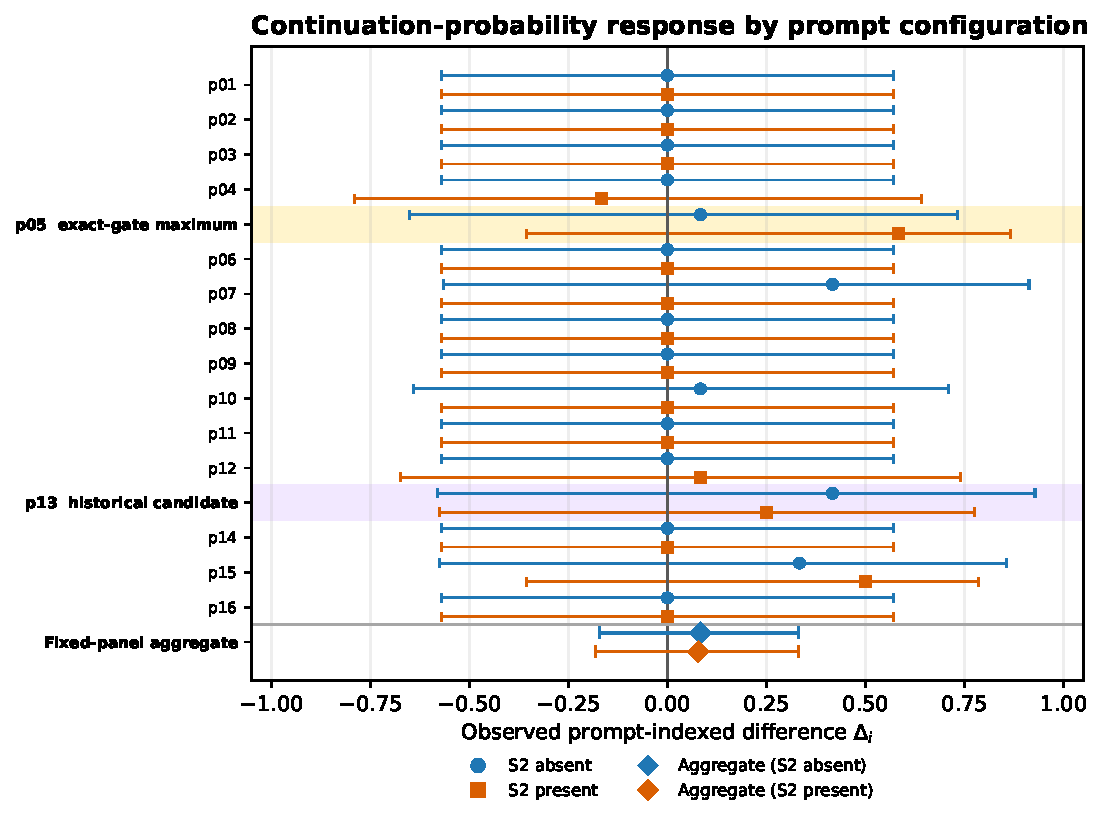
\includegraphics[width=0.95\textwidth,height=\textheight]{figures/prompt-indexed-delta.pdf}

\emph{Figure 1. Prompt-indexed differences in round-one cooperation,
\(\Delta_i=\hat p_i(\delta=.90)-\hat p_i(\delta=.10)\), for both wording
families. Bars are conservative exact simultaneous 95\% intervals with
complete episodes as the unit; observed corners retain non-zero
uncertainty. Blue and orange diamonds show the S2-absent and S2-present
fixed-panel aggregates, respectively. Rows at \(\Delta_i=0\) can reflect
boundary concentration in both recorded cells and are not precise
evidence of no response.}

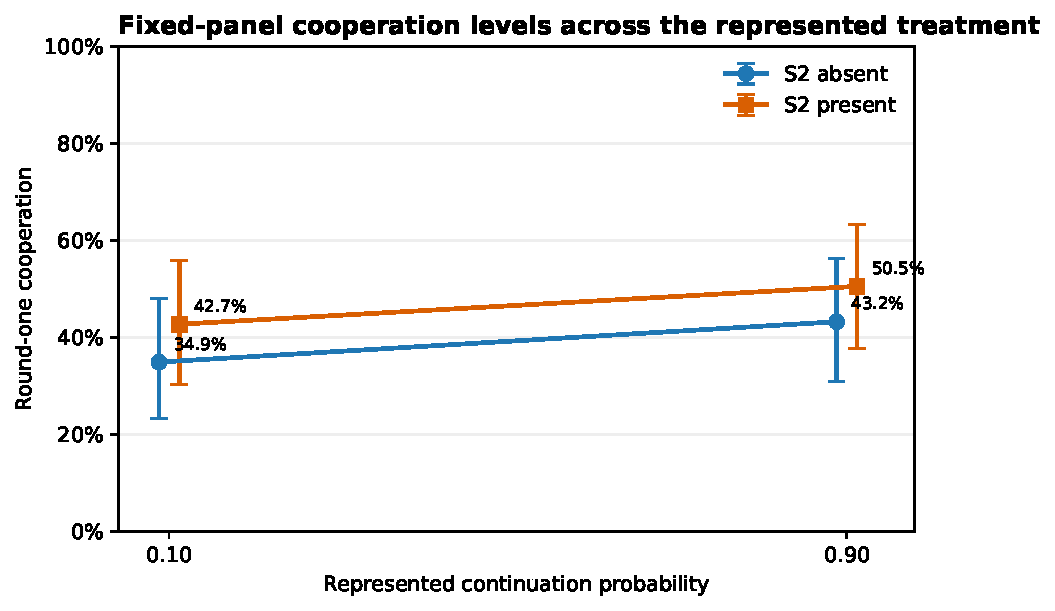
\includegraphics[width=0.95\textwidth,height=\textheight]{figures/condition-means.pdf}

\emph{Figure 2. Fixed-panel cooperation by represented
continuation-probability condition. Error bars are conservative exact
condition intervals; lines connect conditions for orientation only.}

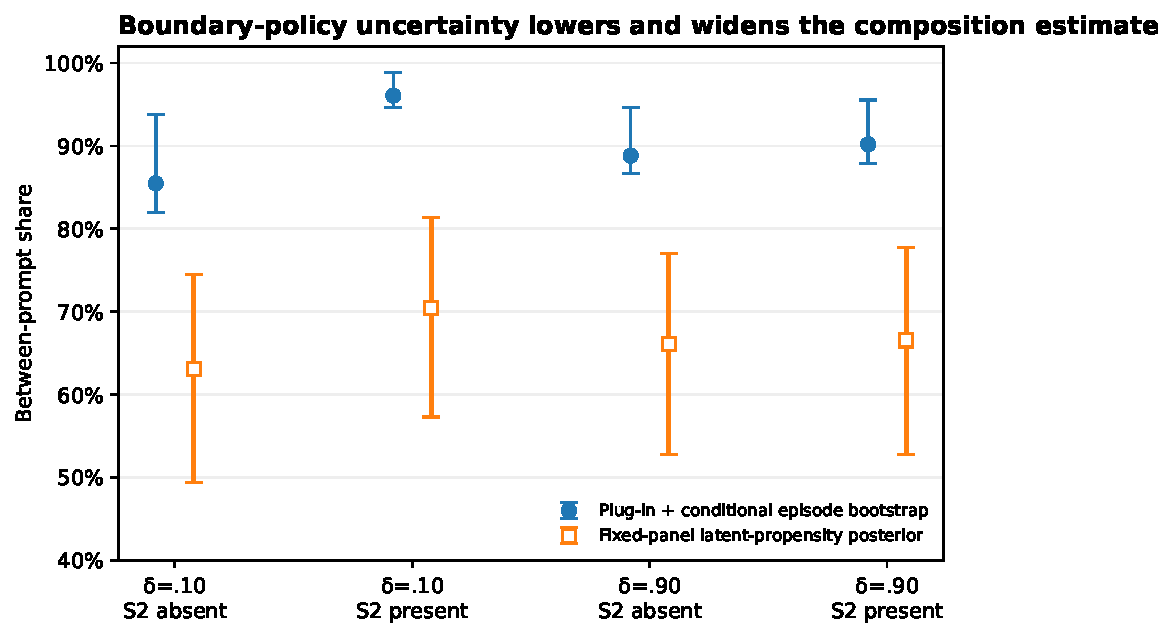
\includegraphics[width=0.95\textwidth,height=\textheight]{figures/between-prompt-share.pdf}

\emph{Figure 3. Between-prompt share of episode-level variation. The
uncertainty-propagating Dirichlet--Jeffreys fixed-panel posterior is the
primary interpretive sensitivity; plug-in/conditional-bootstrap
estimates are shown as a complementary description of the archived
concentration. The two-stage prompt bootstrap changes the estimand and
is reported in text.}

Across all six Phase 5 conditions, the historical seat-level rule
classifies 14/96 persona--condition cells interior, the exact episode
projection 11/96, and the Dirichlet--Jeffreys sensitivity 19/96. In the
registered 32-unit set, the counts are 3/32, 2/32, and 5/32. At n=6 with
a three-valued discrete outcome, modest differences in interval width
deterministically move cells across the threshold; the divergence
reflects both interval construction and low discrete-sample resolution.
The continuous posterior and variance components are therefore more
informative than the binary census.

\hypertarget{what-the-marginal-checks-cannot-identify}{%
\subsubsection{4.2 What the marginal checks cannot
identify}\label{what-the-marginal-checks-cannot-identify}}

Let \(p_i(d)=E[Y\mid i,d]\), where \(i\) indexes the complete explicit
persona prompt and \(d\) the experimental condition.

\textbf{Proposition A: broad bands only partially identify the aggregate
contrast.} If a synthetic condition mean is accepted within tolerance
\(\epsilon_d\) of a reference mean in each condition, then

\[
|\Delta^S-\Delta^H|\le \epsilon_0+\epsilon_1.
\]

Equivalently, accepted bands \([\ell_0,u_0]\) and \([\ell_1,u_1]\) imply
only

\[
\Delta^S\in[\ell_1-u_0,u_1-\ell_0].
\]

Exact condition-specific mean matching would force the aggregate effect
by the identity \(\Delta=\mu_1-\mu_0\); the empirical failure lives in
the slack of coarse criteria.

\textbf{Proposition B: aggregate moments do not identify microstructure
or response coupling.} This is an application of the law of total
variance and classical Fréchet--Hoeffding/Sklar coupling results
{[}Hoeffding 1940; Sklar 1959{]} to synthetic-participant validation,
not a new probability theorem. Mean and total variance do not identify
how variation is divided between prompt configurations and repeated
draws, nor do they identify distributional shape or boundary
concentration. Even exact condition-specific distributions do not
identify the cross-condition coupling and therefore do not identify the
distribution of prompt-indexed responses \(\Delta_i=p_i(1)-p_i(0)\).
Reusing an explicit persona string supplies one prompt-indexed coupling,
but interpreting it as a stable synthetic individual's potential-outcome
contrast requires latent-person invariance, which this study does not
test.

The study therefore identifies a composition pattern in one fixed prompt
panel. It does not establish that humans have a different
microstructure, that RLHF caused the pattern, that latent-user drift is
absent, or that the same pattern occurs across persona generators.

\hypertarget{control-channel-interactions}{%
\subsubsection{4.3 Control-channel
interactions}\label{control-channel-interactions}}

For the bare configuration, round-one cooperation was 0.000 at every
registered continuation probability. X2 decomposed the v1 and v2a prompt
bundles into six sentence/block spans and constructed forward and
reverse ladders by replacing one complete span at a time. The selected
S2 operation replaced and repositioned ``After every round there is a
\{deltaPct\}\% chance the session continues with another round'' with
``At the end of each round there is a \{deltaPct\}\% chance that the
session goes on for one more round.'' Screening used ten episodes per
rung; the selected minimal pair was confirmed at temperature 0.7 on 20
fresh episodes per side (seeds 2953--2972), moving cooperation from 0/40
to 37/40. Because wording and position were one atomic operation, the
design does not separate them.

In the label-swap cell, canonical payoffs were held fixed while
``Cooperate'' and ``Defect'' were attached to opposite strategic roles.
The bare configuration chose the cooperation-worded option 0/40 times
and instead took the payoff-dominated role whenever it carried the word
``Defect.'' This shows that the displayed label or a label-linked
learned prior can override payoff dominance in this registered cell. It
does not identify intrinsic lexical valence: a learned game-theoretic
association such as ``Defect = equilibrium/dominant action in Prisoner's
Dilemma'' is an equally plausible mechanism. A structurally equivalent
non-PD control retaining the same labels was not run.

Persona conditioning produces two observed contrasts, but they are not
factorially separable. Differences among complete persona prompts
generate the leaning gaps reported in §4.1. Adding any tested persona
string reverses the bare swap-cell choice, yet no non-semantic prefix
matched for length, punctuation, and position was run; semantic persona
content cannot be isolated from generic sequence-format disruption. In
the swap cell, label and payoff also point to the same option for
persona-conditioned configurations, leaving the reversal mechanism
ambiguous.

P5-3(b)'s 24 evaluable lanes comprise sixteen personas at T=0.7 plus
p02, p06, p11, and p15 at each of T=1.0 and T=1.3. Every lane retains a
simultaneous episode-exact lower bound above the frozen 0.20 threshold;
the minimum is 0.462. The pooled P5-2 task-consistent share is 90/704
seat decisions across 352 episodes, equivalently 45/352=0.128 on episode
means. The frozen historical adjudication used the seat-level rule. An
episode-iid Clopper--Pearson projection gives {[}0.092, 0.172{]}, but
that interval does not propagate the prompt clustering visible elsewhere
in the study. Two post-adjudication, zero-call sensitivities retain the
historical point estimate while changing the uncertainty model: a
stratified prompt-cluster bootstrap over the forty registered persona ×
conflict-cell clusters gives 95\% interval {[}0.071, 0.189{]}, and a
fixed-panel Dirichlet--Jeffreys latent-propensity aggregation gives
posterior median 0.172 with 95\% interval {[}0.152, 0.195{]}. Both
remain below the registered 0.20 persona-dominant boundary, although the
Bayesian result approaches it. Every repeated conflict subcell is mixed;
only the swap cell is individually persona-dominant. The pooled
classification is therefore mechanism-confounded and carried by the swap
cell, not evidence of a general persona-dominance mechanism.

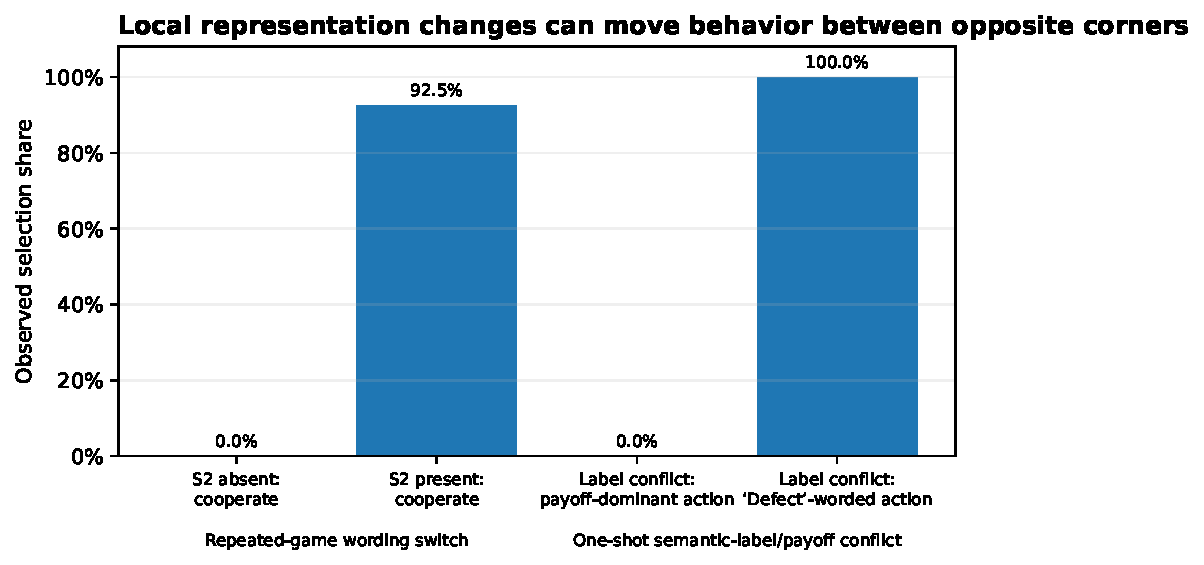
\includegraphics[width=0.95\textwidth,height=\textheight]{figures/representation-effects.pdf}

\emph{Figure 4. Two representation interventions in the bare
configuration. The S2 wording-and-position operation moved cooperation
from 0/40 to 37/40. In the one-shot label conflict, the payoff-dominant
action was never chosen when the dominated role carried ``Defect.''
These bars report selection shares, not a common or uniquely identified
causal mechanism.}

\hypertarget{the-favored-persona-level-result-is-not-prospectively-confirmed-the-archived-family-is-underpowered}{%
\subsubsection{4.4 The favored persona-level result is not prospectively
confirmed; the archived family is
underpowered}\label{the-favored-persona-level-result-is-not-prospectively-confirmed-the-archived-family-is-underpowered}}

Under the historical seat-level rule, persona p13 moved from 0.333
cooperation at δ=.10 to 0.750 at δ=.90 and passed a per-candidate
lower-bound test. The rule searched multiple persona × wording
candidates and fired on any pass without declared family-level error
control. External review identified that defect.

Three 200,000-permutation gate constructions are now reported; all
permutation p-values use the add-one convention,
\(\widehat p=(r+1)/(B+1)\), with exact Monte Carlo intervals. Under the
historical seat-level gate, p13 remains the maximum at +0.4167, with
familywise \(p=0.059230\), Monte Carlo 95\% interval {[}0.058194,
0.060268{]}. Under the percentile episode-cluster-bootstrap sensitivity,
p13 also remains the maximum and \(p=0.043455\), interval {[}0.042561,
0.044353{]}. The exact projection is the conservative reference because
it has finite-sample coverage for the discrete episode mean; the
percentile bootstrap is retained symmetrically but has no comparable
small-sample coverage guarantee. Under the conservative exact-episode
gate, p13 is ineligible: its low-δ lower bound falls below 0.05 and its
high-δ upper bound exceeds 0.95. Only p04/s2p and p05/s2a pass both
gates; the largest eligible slope belongs to p05/s2a (+0.0833), with
familywise \(p=0.773206\), interval {[}0.771363, 0.775039{]}.

For p13/s2a, the percentile bootstrap admitted both conditions as
interior---δ=.10: {[}0.083, 0.667{]}; δ=.90: {[}0.583,
0.917{]}---whereas the conservative exact projection rejected
both---{[}0.047, 0.800{]} and {[}0.287, 0.954{]}, respectively. Neither
recorded cell was at an exact corner. The eligibility difference
therefore arises from small-sample interval width and coverage behavior,
not from a corner interval falsely passing the gate.

The complete data-dependent gate is dynamically reapplied within every
permutation, not frozen from the observed-data mask. The implementation
precomputes 56 possible-composition gate values and performs 25,600,000
condition-gate lookup applications at B=200,000. In a deliberately
incorrect comparison that froze the observed-data mask, the maximum
statistic differed from the dynamic procedure in 718 of 5,000 null draws
(14.4\%), showing that reapplication materially changes the reference
distribution. Lookup/direct parity and the regression are recorded in
\texttt{docs/analysis/submission/round5/round5-review-audit.md}.

An exhaustive attainability audit shows that, with six episodes per
condition, 12 of the 28 possible episode-value compositions pass the
exact gate. Their sample means range from 0.333 to 0.667, but
eligibility depends on the full \({0,0.5,1}\) composition rather than on
the mean alone. Two eligible cells can therefore differ by at most
0.333. Under the archived 32-candidate null structure, the add-one
familywise tail probability at that maximum attainable slope is
0.075040, with Monte Carlo 95\% interval {[}0.073884, 0.076198{]}; no
exact-gate result in this archived family can reach 0.05. The exact
analysis is therefore a valid dependence-aware sensitivity but not a
powered disconfirmation of a p13-sized capability claim. The record
neither prospectively confirms nor decisively disconfirms p13; it
identifies a replication target whose next test must be sized
prospectively (Appendix A.4). A Phase 6 test will preregister the
candidate family, episode-level dependence unit, interiority gate,
maximum statistic, familywise decision rule, and sample size before any
data are collected.

These variants were specified and executed together only after external
review exposed the original defects. No familywise gate was registered
at the original freeze, and the repository contains no
seal-before-compute record for these sensitivities. The analyses ran in
GitHub Actions against archived databases with fixed seeds, and their
outputs were committed regardless of direction. Accordingly, the
favorable \(p=0.043455\) variant cannot create prospective confirmation,
just as the other variants cannot retroactively strengthen the frozen
claim. The historical mechanical P5-3 verdict remains visible because
clause (b) fired strongly and p13 passed the rule as frozen.
Scientifically, p13 is a replication target, not a finding. Clause (a)
did not prospectively establish the capability claim because the frozen
search lacked family control; the conservative post-adjudication
procedure is too underpowered at n=6 to provide decisive evidence
against it.

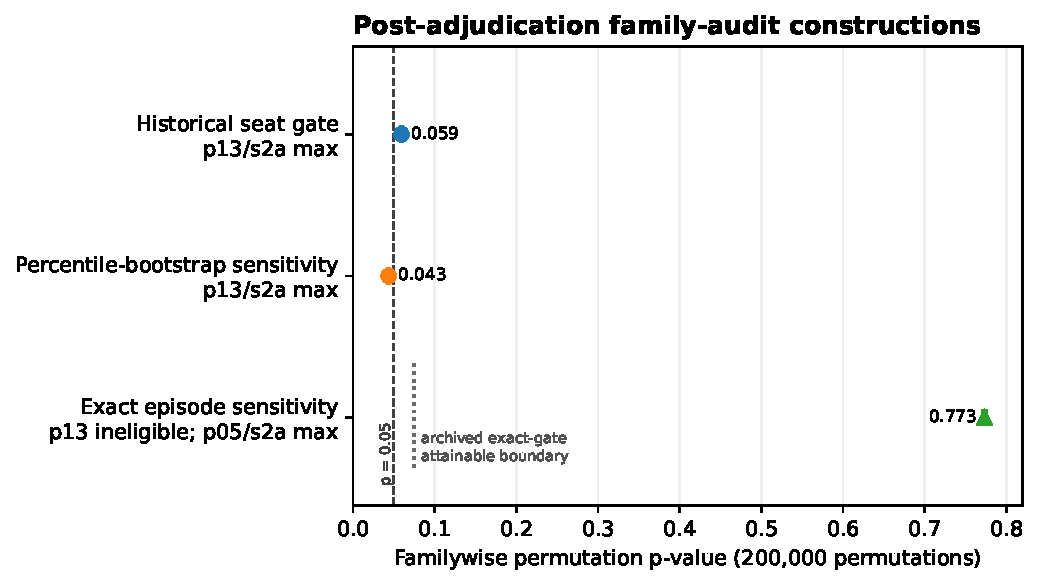
\includegraphics[width=0.95\textwidth,height=\textheight]{figures/p13-audit.pdf}

\emph{Figure 5. Post-adjudication familywise constructions. The first
two points are p13/s2a under the historical and percentile-bootstrap
gates. Under the conservative exact-episode gate, p13 is ineligible; the
third point is the familywise result for the largest eligible candidate,
p05/s2a. The dotted line at \(p=0.075040\) marks the estimated minimum
attainable familywise p-value for the archived \(n=6\), 32-candidate
exact-gate design and applies only to that construction. None of the
procedures was registered at the original freeze; no point creates
prospective confirmation.}

\hypertarget{auditability}{%
\subsubsection{4.5 Auditability}\label{auditability}}

Twelve registered author predictions were refuted by data and published.
Four underspecified analysis choices were resolved outcome-blind. A
two-sided gate blocked a false ceiling conclusion. Sentinels detected a
time-indexed behavioral discontinuity in an unversioned endpoint and
exposed a monitoring gap that was repaired with an attestation gate. The
public capsule now verifies all 4,916 confirmatory Phase 3--5 runs with
zero live model calls: 4,896 LLM runs replay byte-exact and 20
deterministic baselines are independently recomputed. External review
then found the family-error and dependence defects discussed above; the
archived record made both diagnosable and correctable.

The claim is bounded: the machinery is procedurally exact and
extensively auditable. Its strongest achievement is not self-validation
but preservation of enough provenance for outsiders to identify where
procedural correctness stopped short of statistical validity.

\hypertarget{discussion}{%
\subsection{5. Discussion}\label{discussion}}

\hypertarget{implications}{%
\subsubsection{5.1 Implications}\label{implications}}

For synthetic-participant practice, broad marginal resemblance is a weak
validation target. Lightweight conditioning can generate plausible
aggregate levels and substantial cross-prompt dispersion while yielding
small observed treatment-response point estimates whose uncertainty
remains wide. Validation should therefore report response surfaces over
declared interventions and representation families, together with
assay-sensitivity checks, dependence-aware uncertainty, model/provider
provenance, and temporal monitoring. Statistical calibration {[}Hullman
et al.~2026{]}, causal-surrogacy assumptions {[}Persson et al.~2026{]},
and latent-drift diagnostics {[}Lin et al.~2026{]} are complementary
rather than competing safeguards.

The result can be read as a synthetic-subject analogue of the
reduced-form/structural distinction associated with the Lucas critique
{[}Lucas 1976{]}: fitting or selecting for aggregate resemblance need
not identify behavior under a changed treatment. In psychometric terms,
it is a construct-validity and assay-sensitivity problem {[}Cronbach \&
Meehl 1955; ICH E10; Temple \& Ellenberg 2000{]}. Agent-based modeling's
equifinality and pattern-oriented validation provide a related analogy
{[}Windrum et al.~2007; Grimm et al.~2005{]}. These are organizing
analogies, not claims that the study literally estimates a structural
economic model or validates a human measurement model.

The results also show why binary certification language should be used
sparingly. The historical P5-1a predicate passes under its frozen
seat-level rule and under the conservative episode-exact interval, but
fails under a reasonable Dirichlet--Jeffreys sensitivity. The underlying
continuous evidence is clearer than the thresholded label: plug-in
estimates condition on empirical boundary concentration and therefore
tend upward, whereas the Jeffreys posterior shrinks six-episode corner
cells toward the interior and therefore tends downward. These views
bracket the composition claim under opposite conditioning choices rather
than compete as interchangeable estimates; the posterior medians remain
above one-half while the lowest 95\% bound crosses it.

For deployment, behavior that can be rewritten by a sentence, an action
token, or an identity prefix is safety-relevant. The label-conflict
result does not show that lexical valence always dominates incentives:
numerical payoffs move behavior in other cells, and the observed choice
may reflect semantic framing, learned game-theoretic priors, or their
interaction.

\hypertarget{the-precommitted-discussion-and-what-changed-after-review}{%
\subsubsection{5.2 The precommitted discussion, and what changed after
review}\label{the-precommitted-discussion-and-what-changed-after-review}}

The Phase 5 discussion was sealed before its data existed. Excerpt (full
text in supplement; sha \texttt{1f1d7de9…e356}):

\begin{quote}
``The headline of Phase 5 is an existence result the program registered
against itself: at least one persona in the sealed sixteen passed the
two-sided assay gate and showed the registered signature of incentive
sensitivity. The author's registered prediction---that none would---is
refuted, and the refutation is the finding. \ldots{} The capability was
recoverable by content-side conditioning\ldots{} The scope of the claim
is deliberately narrow.''
\end{quote}

\begin{longtable}[]{@{}
  >{\raggedright\arraybackslash}p{(\columnwidth - 2\tabcolsep) * \real{0.5000}}
  >{\raggedright\arraybackslash}p{(\columnwidth - 2\tabcolsep) * \real{0.5000}}@{}}
\toprule\noalign{}
\begin{minipage}[b]{\linewidth}\raggedright
Precommitted interpretation
\end{minipage} & \begin{minipage}[b]{\linewidth}\raggedright
Current status after external review and zero-call reanalysis
\end{minipage} \\
\midrule\noalign{}
\endhead
\bottomrule\noalign{}
\endlastfoot
At least one persona establishes an unconfounded incentive-response
existence result & \textbf{Not prospectively established.} The frozen
search lacked family control, and the post-adjudication procedures were
method-dependent and unregistered. The conservative exact procedure
cannot reach conventional familywise rejection in the archived n=6
design. See §4.4; p13 remains a replication target. \\
``No game-relevant instruction---trait words only'' & Restated
precisely: no explicit game terminology, action recommendation, or
payoff reference; traits are strategically relevant information, and
name, age, and occupation are uncontrolled semantic treatments. \\
Persona framing ``contested or beat'' task switches & Pooled choice
result survives exact episode inference, but every repeated conflict
subcell is mixed; the pooled dominance classification is entirely
carried by the word/payoff-confounded swap cell. \\
Bare corners characterize the configuration rather than the model's
capability envelope & Retained only as a future hypothesis. The p13
evidence no longer supports it; clause (b) demonstrates a robust choice
reversal but does not identify incentive sensitivity. \\
\end{longtable}

The sealed text remains unchanged because its evidentiary value lies
partly in making interpretive error visible. The correction is additive
and explicit rather than silently rewritten.

\hypertarget{limitations}{%
\subsection{6. Limitations}\label{limitations}}

The confirmatory predicates were registered and adjudicated separately
at nominal thresholds; no study-wide alpha allocation or familywise rule
was registered across P5-1a, P5-1b, P5-2, P5-3(a), P5-3(b), and the
sequential X1 extension. They address distinct estimands and are not
interpreted here as one omnibus test, but study-level false-positive
exposure is consequently greater than under a prospectively hierarchical
or alpha-spending design. A Phase 6 replication should preregister the
primary/secondary hierarchy, candidate families, dependence units,
maximum statistics, and cross-predicate error allocation before data
collection.

The primary evidence comes from one deployment and sixteen complete
prompt bundles. Generalization to a persona generator, other models, or
human participants is not identified. The uncertainty views answer
different questions: the latent-propensity posterior is prior-dependent,
the plug-in/conditional bootstrap conditions on recorded boundary
concentration, and the two-stage bootstrap changes the estimand by
resampling prompts.

The treatment-response intervals are wide because each prompt-cell has
six independent episodes and the exact projection retains uncertainty at
empirical corners. The binary interior census is correspondingly
sensitive to small-n discrete interval width. Explicit persona strings
are paired across conditions, but latent-person invariance is untested.
The continuation process was manipulated together with its textual
representation. The persona-prefix contrast lacks a format-matched
neutral control. The label-swap result cannot distinguish semantic
valence from memorized game-theoretic associations because no non-PD
control retained the same labels.

The registered choice-entropy secondary is defined and reported in
Appendix A.1. Its matched-lattice decline survives composition matching,
but unequal seat counts imply slightly different finite-sample plug-in
bias across temperatures; the comparison is exploratory, mechanism-free,
and does not isolate temperature from persona conditioning. The
high-temperature continuation interaction was not registered, and the
Gemini tier is descriptive under endpoint non-stationarity.

Human references are published and protocol-nonmatched. The original
familywise analyses were specified after review and cannot create
retrospective confirmation. The exact n=6 family is underpowered by
construction; p13 remains a replication target, not evidence for or
against a general capability envelope.

\hypertarget{reproducibility-and-data-availability}{%
\subsection{7. Reproducibility and data
availability}\label{reproducibility-and-data-availability}}

The public repository contains the event stores, prompt registries,
sealed registrations, adjudication records, timestamp proofs,
post-adjudication analyses, figures, manuscript history, and review
record. The one-command capsule verifies all 4,916 confirmatory Phase
3--5 runs with zero credentials and zero live model calls. The audit
covers 320 registered Phase 3/X1 LLM runs, 20 deterministic Phase 3
baselines, 2,864 Phase 4 runs, and 1,712 Phase 5 runs; three additional
completed legacy entry/diagnostic runs are also replayed but are not
counted as confirmatory. Phase 3 replay re-renders every prompt,
requires recorded-cache hash hits, reparses raw completions, recomputes
actions, payoffs, and RNG draw counts, and checks recorded call parity.
The deterministic P3-C3 baseline is independently recomputed from
archived seeds and game objects.

Phase 3 used a legacy provider path without Phase 4--5 response IDs or
deterministic request-body SHA capture. Phase 4--5 contain 30,421 normal
request events and 30,397 response events; the 24-event difference is
the disclosed provider-failure partial set. Each partial belongs to a
failed run, was excluded from completed-run analyses and the 4,916-run
replay denominator, and was never decoded as an action. Request attempts
remain represented in request and budget accounting rather than being
silently discarded; only completed replacement runs, where present under
the registered replacement procedure, enter analysis. Those response
records contain rendered prompts, bundle and request-body hashes, engine
commit and provider route, raw text, and provider response IDs.
Individual completion payloads were not provider-attested or separately
hash-chained at receipt. Capsule checksum manifests and external
timestamps make the released database snapshot tamper-evident relative
to publication; replay cannot prove that no alteration occurred before
snapshot sealing.

Reproduce the confirmatory record with:

\begin{Shaded}
\begin{Highlighting}[]
\FunctionTok{git}\NormalTok{ clone https://github.com/yoheinakajima/synthetic{-}players}
\BuiltInTok{cd}\NormalTok{ synthetic{-}players/capsule}
\FunctionTok{bash}\NormalTok{ verify.sh}
\end{Highlighting}
\end{Shaded}

All post-adjudication analyses are zero-call scripts over the archived
databases and are labeled separately from prospectively registered
results.

\hypertarget{attribution}{%
\subsection{8. Attribution}\label{attribution}}

The human author selected the research questions, approved the
registered designs, adjudicated which reviewer recommendations to adopt,
and accepts responsibility for every claim. The autonomous pipeline
executed registration, dispatch, adjudication, and replay as apparatus.
AI reviewers supplied adversarial analysis that materially changed the
manuscript, including the family-error diagnosis, the condition-mean
identity, the dependence-unit critique, and the latent-person-invariance
correction.

The role of one round-2 reviewer subsequently expanded from critique to
specification of the post-adjudication analyses and management of their
integration. Those analyses were executed by GitHub Actions against the
archived databases; resulting commits were authored by Yohei Nakajima or
the Actions bot. A later reviewer independently checked the branch
through an anonymous blobless clone against the generated JSON and
commit history. Review prompts, role changes, adopted recommendations,
and the independent verification memo are archived under
\texttt{docs/reviews/}. AI systems are not listed as authors. Their
roles as research apparatus and adversarial reviewers are disclosed here
and in the public review record; the human author accepts responsibility
for every claim.

\begin{center}\rule{0.5\linewidth}{0.5pt}\end{center}

\hypertarget{appendix-a-supplementary-scope-and-prospective-design}{%
\subsection{Appendix A --- Supplementary scope and prospective
design}\label{appendix-a-supplementary-scope-and-prospective-design}}

\hypertarget{a.1-temperature-secondary}{%
\subsubsection{A.1 Temperature
secondary}\label{a.1-temperature-secondary}}

Choice entropy is defined as base-2 Shannon entropy,
\(H=-\sum_a p(a)\log_2p(a)\), over round-one payoff-role choices. The
historical registered secondary pooled all valid choices at each
temperature, but the T=0.7 and higher-temperature samples had different
composition. The matched-sweep reanalysis uses only persona-cell lanes
observed at all three temperatures:

\begin{longtable}[]{@{}
  >{\raggedleft\arraybackslash}p{(\columnwidth - 8\tabcolsep) * \real{0.2000}}
  >{\raggedleft\arraybackslash}p{(\columnwidth - 8\tabcolsep) * \real{0.2000}}
  >{\raggedleft\arraybackslash}p{(\columnwidth - 8\tabcolsep) * \real{0.2000}}
  >{\raggedleft\arraybackslash}p{(\columnwidth - 8\tabcolsep) * \real{0.2000}}
  >{\raggedleft\arraybackslash}p{(\columnwidth - 8\tabcolsep) * \real{0.2000}}@{}}
\toprule\noalign{}
\begin{minipage}[b]{\linewidth}\raggedleft
temperature
\end{minipage} & \begin{minipage}[b]{\linewidth}\raggedleft
matched units
\end{minipage} & \begin{minipage}[b]{\linewidth}\raggedleft
seats
\end{minipage} & \begin{minipage}[b]{\linewidth}\raggedleft
pooled Shannon entropy (bits)
\end{minipage} & \begin{minipage}[b]{\linewidth}\raggedleft
mean within-unit entropy (bits)
\end{minipage} \\
\midrule\noalign{}
\endhead
\bottomrule\noalign{}
\endlastfoot
0.7 & 13 & 544 & 0.8310 & 0.4484 \\
1.0 & 13 & 284 & 0.7822 & 0.2566 \\
1.3 & 13 & 284 & 0.7698 & 0.2877 \\
\end{longtable}

The registered pooled decline is partly composition-confounded but
survives on the identical sweep lattice. Mean within-unit entropy is
reported separately because pooled entropy can remain high when
different prompt-cell units occupy opposite boundaries. Neither
statistic identifies a temperature mechanism. The plug-in Shannon
estimates use unequal seat counts (544 versus 284 and 284), so their
small finite-sample biases are not identical; no bias-corrected entropy
claim is made.

\hypertarget{a.2-other-supplementary-findings}{%
\subsubsection{A.2 Other supplementary
findings}\label{a.2-other-supplementary-findings}}

RPS retained a role-attached rock bias after neutral symbols and
randomized order, with a cross-vendor sign reversal. The adversary suite
showed opponent-contingent sequential structure. A sentinel case study
documents endpoint drift and the resulting monitoring repair. These
results and the Claude Haiku entry-gate failure remain in the public
supplementary record but are outside the main causal arc.

\hypertarget{a.3-prospective-replication}{%
\subsubsection{A.3 Prospective
replication}\label{a.3-prospective-replication}}

A Phase 6 replication will preselect one target or a small candidate
family and preregister the complete familywise procedure: candidate set,
episode-level unit, interiority gate, maximum statistic, decision
threshold, and sample size. It should also include a format-matched
neutral prefix, a continuation-probability × wording factorial, and a
structurally equivalent non-PD label-conflict control. The registered
power calculation must simulate the exact decision rule under its
declared dependence model rather than reuse the archived 32-candidate
search.

\hypertarget{a.4-research-record}{%
\subsubsection{A.4 Research record}\label{a.4-research-record}}

The complete correction ledger, sealed discussion text, dead-predictions
ledger, reviewer-role disclosures, and mechanical review disposition
matrices are maintained in \texttt{docs/reviews/} and
\texttt{docs/analysis/submission/}. Historical artifacts are never
silently rewritten; current interpretations are linked to the versions
they amend.

\hypertarget{references}{%
\subsection{References}\label{references}}

\begingroup
\small
\setlength{\parskip}{0.30em}

Berger, J. O., Bernardo, J. M., and Sun, D. (2009). The formal
definition of reference priors. \emph{Annals of Statistics, 37}(2),
905--938. https://doi.org/10.1214/07-AOS587

Efron, B., and Tibshirani, R. J. (1993). \emph{An Introduction to the
Bootstrap}. Chapman \& Hall/CRC.
https://doi.org/10.1007/978-1-4899-4541-9

Holtzman, A., Buys, J., Du, L., Forbes, M., and Choi, Y. (2020). The
curious case of neural text degeneration. In \emph{International
Conference on Learning Representations}.

Clopper, C. J., and Pearson, E. S. (1934). The use of confidence or
fiducial limits illustrated in the case of the binomial.
\emph{Biometrika, 26}(4), 404--413.
https://doi.org/10.1093/biomet/26.4.404

Hoeffding, W. (1940). Maßstabinvariante Korrelationstheorie.
\emph{Schriften des Mathematischen Instituts und des Instituts für
Angewandte Mathematik der Universität Berlin, 5}, 181--233.

Lehmann, E. L., and Romano, J. P. (2005). \emph{Testing Statistical
Hypotheses} (3rd ed.). Springer. https://doi.org/10.1007/0-387-27605-X

Sklar, A. (1959). Fonctions de répartition à n dimensions et leurs
marges. \emph{Publications de l'Institut de Statistique de l'Université
de Paris, 8}, 229--231.

Westfall, P. H., and Young, S. S. (1993). \emph{Resampling-Based
Multiple Testing: Examples and Methods for p-Value Adjustment}. Wiley.

Akata, E., Schulz, L., Coda-Forno, J., Oh, S. J., Bethge, M., and
Schulz, E. (2025). Playing repeated games with large language models.
\emph{Nature Human Behaviour, 9}, 1380--1390.
https://doi.org/10.1038/s41562-025-02172-y

Anthis, J. R., Liu, R., Richardson, S. M., Kozlowski, A. C., Koch, B.,
Brynjolfsson, E., Evans, J., and Bernstein, M. S. (2025). Position: LLM
social simulations are a promising research method. \emph{Proceedings of
the 42nd International Conference on Machine Learning, PMLR 267},
81005--81034. https://proceedings.mlr.press/v267/anthis25a.html

Argyle, L. P., Busby, E. C., Fulda, N., Gubler, J. R., Rytting, C., and
Wingate, D. (2023). Out of one, many: Using language models to simulate
human samples. \emph{Political Analysis, 31}(3), 337--351.
https://doi.org/10.1017/pan.2023.2

Ashokkumar, A., Hewitt, L., Ghezae, I., and Willer, R. (2026). Large
language models can predict the results of social science experiments.
\emph{Nature}. https://doi.org/10.1038/s41586-026-10742-x

Batzner, J., Stocker, V., Tang, B., Natarajan, A., Chen, Q., Schmid, S.,
and Kasneci, G. (2025). Whose personae? Synthetic persona experiments in
LLM research and pathways to transparency. \emph{Proceedings of the
AAAI/ACM Conference on AI, Ethics, and Society, 8}(1), 343--354.
https://doi.org/10.1609/aies.v8i1.36553

Bisbee, J., Clinton, J. D., Dorff, C., Kenkel, B., and Larson, J. M.
(2024). Synthetic replacements for human survey data? The perils of
large language models. \emph{Political Analysis, 32}(4), 401--416.
https://doi.org/10.1017/pan.2024.5

Boelaert, J., Coavoux, S., Ollion, É., Petev, I., and Präg, P. (2025).
Machine bias: How do generative language models answer opinion polls?
\emph{Sociological Methods \& Research, 54}(3), 1156--1196.
https://doi.org/10.1177/00491241251330582

Cronbach, L. J., and Meehl, P. E. (1955). Construct validity in
psychological tests. \emph{Psychological Bulletin, 52}(4), 281--302.
https://doi.org/10.1037/h0040957

Dal Bó, P., and Fréchette, G. R. (2011). The evolution of cooperation in
infinitely repeated games: Experimental evidence. \emph{American
Economic Review, 101}(1), 411--429.
https://doi.org/10.1257/aer.101.1.411

Georgousis, D., Lymperaiou, M., Dimitriou, A., Filandrianos, G., and
Stamou, G. (2026). Evaluating counterfactual strategic reasoning in
large language models. arXiv:2603.19167.
https://doi.org/10.48550/arXiv.2603.19167

Grimm, V., Revilla, E., Berger, U., et al.~(2005). Pattern-oriented
modeling of agent-based complex systems: Lessons from ecology.
\emph{Science, 310}(5750), 987--991.
https://doi.org/10.1126/science.1116681

Harry, T., Ngong, I. C., Nweke, C., Feng, Y., and Near, J. (2026).
Beyond fixed psychological personas: State beats trait, but language
models are state-blind. In \emph{Findings of the Association for
Computational Linguistics: ACL 2026}, 26440--26468. Association for
Computational Linguistics.
https://doi.org/10.18653/v1/2026.findings-acl.1316

Horton, J. J. (2023). Large language models as simulated economic
agents: What can we learn from Homo Silicus? NBER Working Paper 31122.
https://doi.org/10.3386/w31122

Hullman, J., Broska, D., Sun, H., and Shaw, A. (2026). This human study
did not involve human subjects: Validating LLM simulations as behavioral
evidence. arXiv:2602.15785. https://doi.org/10.48550/arXiv.2602.15785

International Council for Harmonisation. (2000). \emph{ICH E10: Choice
of control group and related issues in clinical trials}.
https://database.ich.org/sites/default/files/E10\_Guideline.pdf

Li, Y., and Ji, X. (2026). When simulations look right but causal
effects go wrong: Large language models as behavioral simulators.
arXiv:2604.02458. https://doi.org/10.48550/arXiv.2604.02458

Lin, V., Yun, T., Matarić, M. J., Canny, J., Gretton, A., and D'Amour,
A. (2026). The illusion of intervention: Your LLM-simulated experiment
is an observational study. arXiv:2605.20767.
https://doi.org/10.48550/arXiv.2605.20767

Lucas, R. E., Jr.~(1976). Econometric policy evaluation: A critique.
\emph{Carnegie-Rochester Conference Series on Public Policy, 1}, 19--46.
https://doi.org/10.1016/S0167-2231(76)80003-6

Mei, Q., Xie, Y., Yuan, W., and Jackson, M. O. (2024). A Turing test of
whether AI chatbots are behaviorally similar to humans.
\emph{Proceedings of the National Academy of Sciences, 121}(9),
e2313925121. https://doi.org/10.1073/pnas.2313925121

Mousavi Davoudi, S. P., Amiri-Margavi, A., Gholami Davodi, A., Hasani
Balyani, H., and Gharagozlou, A. (2026). Same game, different story: A
minimal conservative strategic robustness benchmark for large language
model agents. arXiv:2607.19670.
https://doi.org/10.48550/arXiv.2607.19670

Pal, S., Mallela, A., Hilbe, C., Pracher, L., Wei, C., Fu, F., Schnell,
S., and Nowak, M. A. (2026). Strategies of cooperation and defection in
five large language models. arXiv:2601.09849.
https://doi.org/10.48550/arXiv.2601.09849

Park, J. S., Zou, C. Q., Kamphorst, J., Egan, N., Shaw, A., Hill, B. M.,
Cai, C., Morris, M. R., Liang, P., Willer, R., and Bernstein, M. S.
(2024, revised 2026). LLM agents grounded in self-reports enable
general-purpose simulation of individuals. arXiv:2411.10109v3.
https://doi.org/10.48550/arXiv.2411.10109

Persson, E., Schultzberg, M., and Ankargren, S. (2026). Statistical
foundations of LLM-based A/B testing: A surrogacy framework for human
causal inference. arXiv:2606.17165.
https://doi.org/10.48550/arXiv.2606.17165

Sclar, M., Choi, Y., Tsvetkov, Y., and Suhr, A. (2024). Quantifying
language models' sensitivity to spurious features in prompt design, or:
How I learned to start worrying about prompt formatting. In
\emph{International Conference on Learning Representations}.

Shanahan, M., McDonell, K., and Reynolds, L. (2023). Role play with
large language models. \emph{Nature, 623}, 493--498.
https://doi.org/10.1038/s41586-023-06647-8

Temple, R., and Ellenberg, S. S. (2000). Placebo-controlled trials and
active-control trials in the evaluation of new treatments. Part 1:
Ethical and scientific issues. \emph{Annals of Internal Medicine,
133}(6), 455--463.
https://doi.org/10.7326/0003-4819-133-6-200009190-00014

Windrum, P., Fagiolo, G., and Moneta, A. (2007). Empirical validation of
agent-based models: Alternatives and prospects. \emph{Journal of
Artificial Societies and Social Simulation, 10}(2), 8.
https://www.jasss.org/10/2/8.html

Xiao, Y., Zhang, V. J., Yang, C., Ma, N., Xuan, W., and Huang, J.-t.
(2026). The chameleon's limit: Investigating persona collapse and
homogenization in large language models. arXiv:2604.24698.
https://doi.org/10.48550/arXiv.2604.24698

Xie, Y., Liang, L., Li, S., Lu, Y., Xiao, Z., Shi, M., Huang, J., Wang,
M., and Xie, Y. (2026). Evaluating the statistical realism of
LLM-generated social science data. \emph{Proceedings of the National
Academy of Sciences, 123}(19), e2538145123.
https://doi.org/10.1073/pnas.2538145123

\endgroup

\end{document}
